\documentclass[10pt]{article}

% Lines beginning with the percent sign are comments
% This file has been commented to help you understand more about LaTeX

% DO NOT EDIT THE LINES BETWEEN THE TWO LONG HORIZONTAL LINES

%---------------------------------------------------------------------------------------------------------

% Packages add extra functionality.
\usepackage{
	times,
	graphicx,
	epstopdf,
	fancyhdr,
	amsfonts,
	amsthm,
	amsmath,
	algorithm,
	algorithmic,
	xspace,
	hyperref,
	multirow,
	tabularx,
	}
\usepackage[left=1in,top=1in,right=1in,bottom=1in]{geometry}
\usepackage{sect sty}	%For centering section headings
\usepackage{enumerate}	%Allows more labeling options for enumerate environments 
\usepackage{epsfig}
\usepackage[space]{grffile}
\usepackage{booktabs}
\usepackage{amsmath}
\usepackage[super]{nth}
\usepackage{array}
\usepackage{graphicx}
\usepackage{enumerate}
\usepackage{alltt}
\usepackage{fancyvrb}
% This will set LaTeX to look for figures in the same directory as the .tex file
\graphicspath{.} % The dot means current directory.

\pagestyle{fancy}

\lhead{\YOURID}
\chead{\MyLang: Language Specification}
\rhead{\today}
\lfoot{CSCI 334: Principles of Programming Languages}
\cfoot{\thepage}
\rfoot{Spring 2022}

% Some commands for changing header and footer format
\renewcommand{\headrulewidth}{0.4pt}
\renewcommand{\headwidth}{\textwidth}
\renewcommand{\footrulewidth}{0.4pt}

% These let you use common environments
\newtheorem{claim}{Claim}
\newtheorem{definition}{Definition}
\newtheorem{theorem}{Theorem}
\newtheorem{lemma}{Lemma}
\newtheorem{observation}{Observation}
\newtheorem{question}{Question}

\setlength{\parindent}{0cm}
%---------------------------------------------------------------------------------------------------------

% DON'T CHANGE ANYTHING ABOVE HERE

% Edit below as instructed
\newcommand{\MyLang}{1 e + a}	% Replace MyLang with your language name #
\newcommand{\PartnerOne}{Valeria Starkova}	% Replace PartnerOne with your name #
\newcommand{\YOURID}{\PartnerOne{}} % Remove \PartnerTwo if working alone.


\title{\MyLang: Language Specification}
\date{Spring 2022}
\author{\PartnerOne{}} % Remove \PartnerTwo if working alone.

\begin{document}
\maketitle

\vspace{\baselineskip}	% Add some vertical space
\graphicspath{ {./images/} }


\maketitle


\section{Introduction}


This language allows drummers to notate drums efficiently, without using inconvenient intermediary software. As it can be tedious to write drum tabs in UIs that are not designed for this purpose, this language lets users write drum tabs in a simple and intuitive way: by utilizing the good old "1 e and a" counting system. 


\item

A drum part's structure is often constant throughout a song, with only slight variations across its parts (intro, verse, pre-chorus, chorus, bridge, etc.). This language also helps to avoid repetition by allowing the user to write one structure only once, then reuse it in other parts with slight modifications if necessary.

\section{Design Principles}

The most important design principle in this language is the fact that users can create and re-use patterns, bars, and beats that can be easily modified when writing the tabs. Perhaps in the future, users will be able to share the source code for each song written in this programming language on a platform similar to GitHub, where they can keep track of their commits, collaborators, etc. Further, the platform will contain a built-in editor and a visual display of the tabs that can be directly played.



\section{Examples}

\subsection{Example 1}
It is very easy to create a pattern, just by using the "1 e and a" counting system. 
We put separators \verb+|+ to disambiguate the division of the beats.
\begin{verbatim}
    time: 4/4
    division: 1/16
    
    title: my title
    subtitle: my subtitle
    
    pattern mypattern : 1 | 2 | 3 | 4 |
    
    render: mypattern
\end{verbatim}

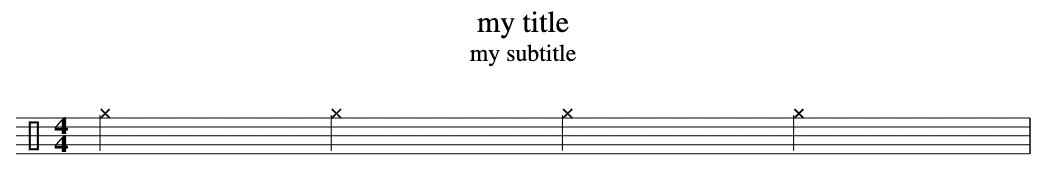
\includegraphics[scale=1.0]{example1.png}


\subsection{Example 2}
Simple example of creating a one measure beat.
\begin{verbatim}
    time :  4/4
    division: 1/16
    
    title: example 2
    subtitle: example 2
    
    pattern mypattern : 1 | 2 | 3 | 4 |
    
    
    bar mybar1:
        hh: [ 1 + | 2  + | 3 + | 4  + | ]
        sn: [ mypattern ]
        bd: [ 1 a | 2 a | 3 a | 4 a |]
    
    
    render: mybar1    
\end{verbatim}
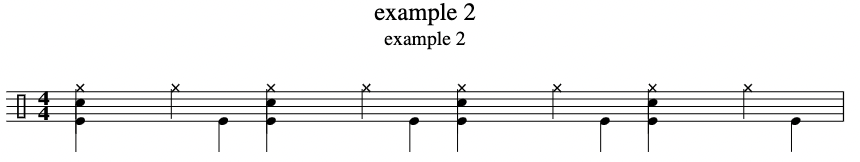
\includegraphics[scale=1.0]{example2.png}

\subsection{Example 3}
Create a beat by repeating the pre-defined measure 4 times and adding a crash cymbal 
on the first beat and changing the pattern of the bass drum. Also repeat the bar 2 times
without any change instructions: 
\begin{verbatim}
    time :  4/4
    division: 1/16
    
    title: example 3
    subtitle: example 3
    
    pattern mypattern : 1 e + a | 2  e + a  | 3 e + a  | 4  e + a  |
    
    bar mybar1:
        hh: [ mypattern ]
        sn: [ | 2 |  | 4 |]
        bd: [ 1 + | 2  + | 3 + | 4 + |]
    
    Snippet mysnippet:
        
        @change 4: 
            mybar1 (1,4) {
                cc: [1 |]
                bd: [ 1 | 2 | 3 | 4 |]
            };
    
        !repeat 2: [ mybar1 ].
    
    render: mysnippet
\end{verbatim}
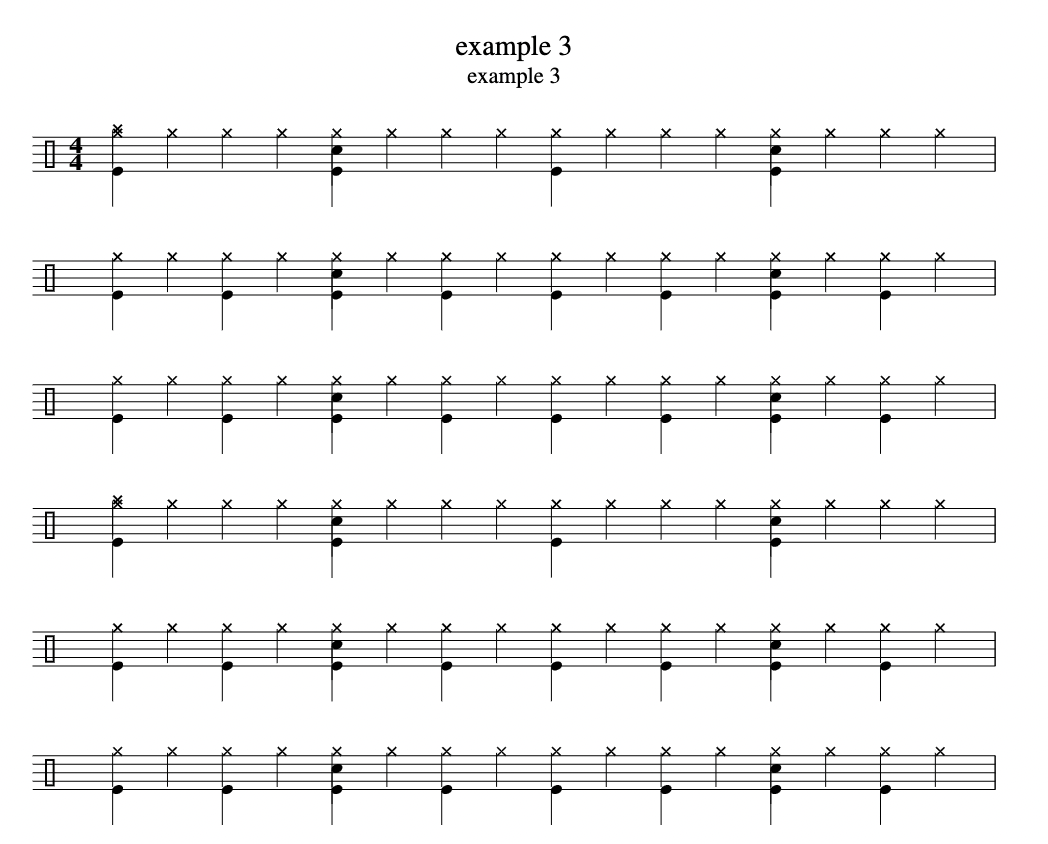
\includegraphics[scale=1.0]{example3.png}

\section{Language Concepts}
There are two core concepts a user should understand in order to write programs in this language. First, how to notate different parts of the drum-set. Below is an example of a basic drum kit and the corresponding abbreviations we will use to write programs.

\begin{verbatim}
CC = Crash cymbal
HH = Hi-hat
RD = Ride cymbal
SN = Snare drum
T1 = High tom
T2 = Low tom
FT = Floor tom
BD = Bass drum
\end{verbatim}

There are also different techniques to play these, such as playing the bell of ride (rd[b]), open hi-hats (o), slightly open hi-hats (\verb+~+), closed hi-hats (hh by default or x), foot hi-hats (\verb+_+), ghost notes (g), flams (f), rimshots (r), accented strokes (a) etc. 

Secondly, a user should be familiar with the “1 e and a” counting system:
\\\\
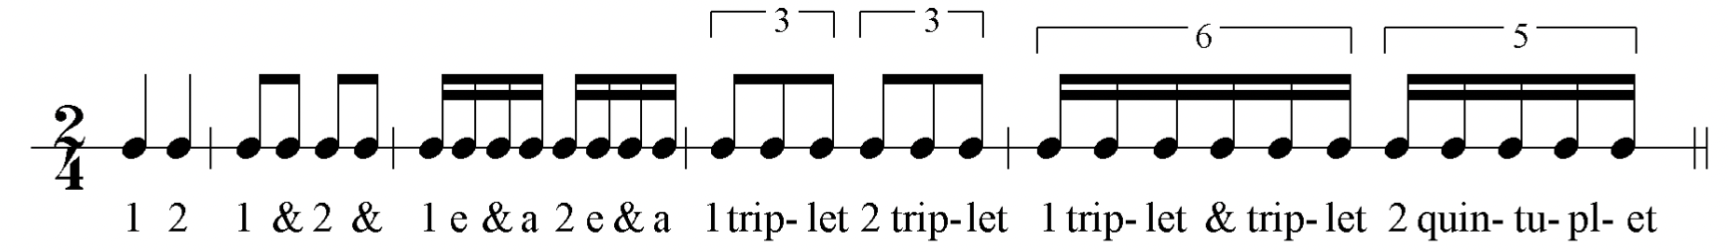
\includegraphics[scale=0.5]{img.png}

Now knowing this, we can assign patterns to each part of the drum kit. For example, in 4/4 time, we can assign to SN (the snare drum) the pattern \verb+1 e | 2 | | 4 a |+, where $|$ just symbolises division of the beat (not necessarily if it is unambiguous).


\section{Syntax}

A pattern is made up of notes. Patterns can be 
assigned to drums in a bar. Bars can be combined to create
a beat. Bars inside a beat can be repeated and modified inside 
a repeat instruction. 
Notes are primitives, which have values 1 e + a.
Patterns have string names.
Bars have string names.
Beats have string names.
Repeat instruction accepts an integer as the value
of how many times to repeat a bar. It also accepts an optional
an argument that represents which bar to modify. Properties to 
modify are specified inside curly brackets. Modifying 
properties is similar to assigned patterns to drums. Can also
keep the pattern the same but change the drum from one to another by 
using the \verb+->+ sign.

\begin{alltt}
    <num>           ::= x \ensuremath{\in} Z+
    <string>        ::= any string
    <varname>       ::= <string> | <num>

    <time>          ::= time: <num>/<num>
    <division>      ::= division: <num>/<num>

    <title>         ::= title: <string>
    <subtitle>      ::= subtitle: <string>
    
    <count>         ::= <num> | e | + | a 
    <sep>           ::= |
    <beat>          ::= <count>+ <sep>
    <pattern>       ::= <beat>+
        
    <pattern_expr>  ::= pattern<varname>: <pattern>
    
    <drums>                 := cc | hh | rd | sn | t1 | t2 | ft | bd
    <drum_pattern_var>      ::= <drums>: <varname>
    <drum_pattern_notes>    ::= <drums>: <pattern>
    <drum_pattern>          ::= [ <drum_pattern_var> | <drum_pattern_notes> ]
                        
    <bar_expr>              ::= bar <varname>: <drum_pattern>+
    
    <repeat>                ::= !repeat <num>: [<varname>+].
    <change_option>         ::= <num> | every <num>
    <change>          ::= $change <change_option>: <varname> (<num>)\ensuremath{\{}<drum_pattern>+\ensuremath{\}};
    <snippet_data>          ::= <repeat> | <change>
    <snippet_expr>          ::= Snippet <varname>: <snippet_data>+

    <render>        ::= render: <varname>

\end{alltt}

\section{Semantics}
\begin{tabularx}{1\textwidth} { 
  | >{\raggedright\arraybackslash}X
  | >{\centering\arraybackslash}X 
  | >{\centering\arraybackslash}X 
  | >{\centering\arraybackslash}X 
  | >{\raggedleft\arraybackslash}X 
  | >{\raggedleft\arraybackslash}X |
  | >{\raggedleft\arraybackslash}X |
  | >{\raggedleft\arraybackslash}X |
  | >{\raggedleft\arraybackslash}X |
  }
 \hline
 Syntax & Abstract Syntax & Type & Meaning \\
 \hline

    % x \in R  & x of int & int & x is a primitive \\
    % \hline
    time: 4/4 & Time of uint8 * uint8 & Settings & Top number tells how many beats should be in one measure, and
    the bottom number tells what value of note should get the beat. \\
    \hline
   
    div: 1/16 & Division of uint8 * uint8 & Settings & The minimum value that notes can divide into \\
    \hline

    title: My Title & Title of string & Settings & Title of the piece \\
    \hline
    
    subtitle: My Subtitle & Subtitle of string & Settings & Subtitle of the piece \\
    \hline

    1 e + a \verb+|+ & Num of int \verb+|+ E \verb+|+  And \verb+|+  A \verb+|+ Sep & Note  & 
    Denotes the division of a note as defined by time signature (bottom number).
    Beats should be separated by \verb+Sep+\\
    \hline
    
    sn & Drum of \verb+|+ CC   \verb+|+ RD     \verb+|+ HH     \verb+|+ SN     \verb+|+ T1   \verb+|+ T2   \verb+|+ BD 
    & Drum 
    & Denotes a drum \\
   \hline

    pattern varname: 1 \verb+|+ 2 e + a \verb+|+ 3 \verb+|+ 4 \verb+|+ & Pattern of PatternName * (Note list) & Pattern & a Pattern is a string denoting the name of the pattern after the keyword 'pattern' and a list of notes after the semicolon\\
    \hline
     hh: string  & Drum * PatternName & DrumPatternVar & pattern variable assigned to a drum after the semicolon  \\
    \hline
     hh: 1 2 3 4  & Drum * (Note list) & DrumPatternNotes & a pattern of notes assigned to a drum after the semicolon  \\
    \hline
     
    
     bar string: 
        hh: [1 \verb+|+ 2 \verb+|+ 3 \verb+|+ 4 \verb+|+]
    
    & Bar of BarName * (DrumPatternVar list * DrumPatternNotes list) & Bar & a Bar is a string denoting the name of the bar after the keyword 'bar' and a list of DrumPatternVar or DrumPatternNotes after the semicolon  \\
    
    \hline

     !repeat <num>: [ varname1 varname2 ].
    
    & Repeat of int * (BarName list) &
    SnippetData & 
    
   repeat instruction will repeat given bars <num> number of times.
    \\
    
    \hline

     @change <num>: varname { cc: [ 1 |] };
    
    & RepeatChange of int * BarName * RepeatOption * (DrumPattern list) &
    SnippetData & 
    
   change instruction behaves similar to repeat in the was that it will
   repeat one bar <num> number of times but it also accepts change instructions 
   inside curly brackets, which are drum->pattern assignments. 
   
   \\
    
    \hline

    Snippet mysnippet: ...
    
    & Snippet of SnippetName * (SnippetData list) &
    Snippet & 
    
   Snippet creates multiple measure long pieces by combining repeat and change 
   instructions.
   \\
    

\end{tabularx}


\begin{enumerate}[i.]
    \item  A primitive value is a note defined by a counting value such as \verb+1+,  \verb+e+,  \verb#+#, \verb+a+.
    \item Values \verb+1+,  \verb+e+,  \verb#+#,  \verb+a+ are combined to create a \verb+pattern+:
    \begin{verbatim}
        pattern: <count>+
    \end{verbatim}
    A \verb+bar+ can be created by applying various \verb+pattern+s to different parts of the drum-set (\verb+hh+, \verb+sn+, \verb+bd+, etc).
    \begin{verbatim}
        bar <string>: 
            <drum>: <pattern>
    \end{verbatim}
    And a \verb+Snippet+ can be created by combining and/or repeating multiple \verb+bar+s. 
    \begin{verbatim}
        Snippet <string>: 
            <bar>
    \end{verbatim}
    \verb+Bar+s can be repeated by "\verb+repeat <num> <bar>+", and the repeated \verb+bar+s can be modified inside curly brackets, where \verb+<bar_num>+ represents the bar number(s) to be modified:
    \begin{verbatim}
        Snippet <string>:
            repeat <num> <bar> (<bar_num>) {
                <drum>: <pattern>
            }
    \end{verbatim}
    Where \verb+<bar_num>+ represents the bar number(s) to be modified.
    \item Diagram representation of my program:
    \\
    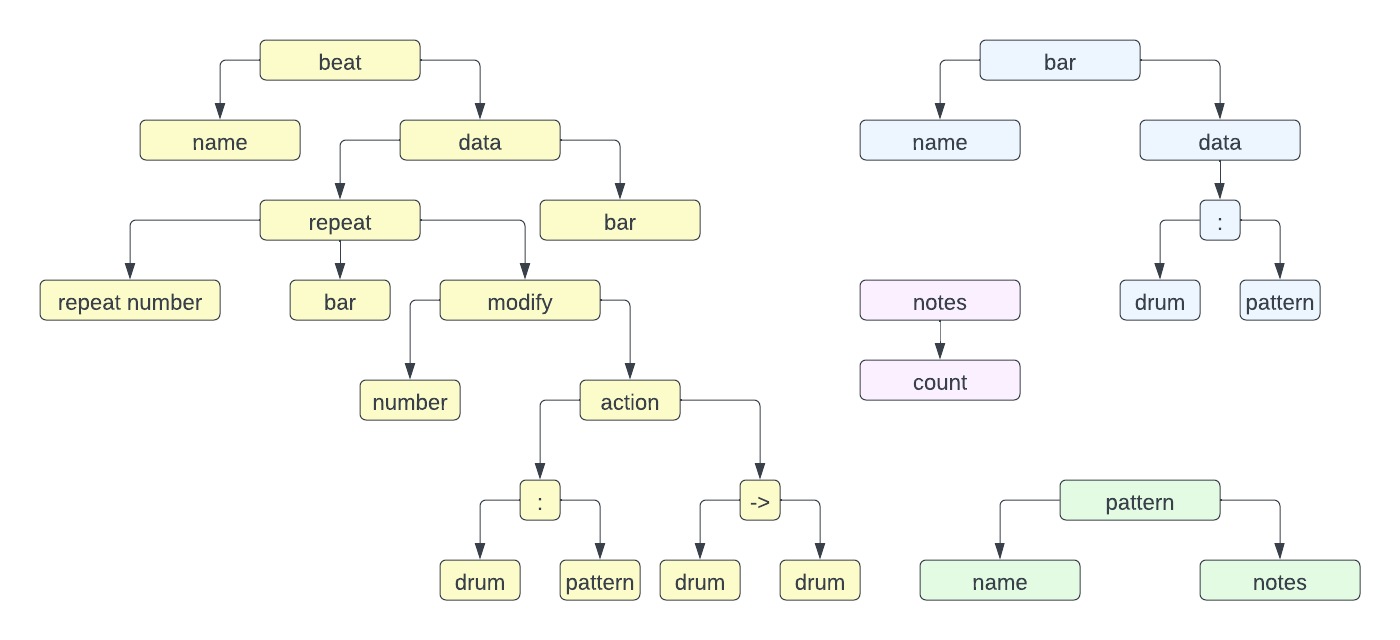
\includegraphics[scale=0.8]{Blank diagram.png}
    
    \item 


	AST for example 1:
    
    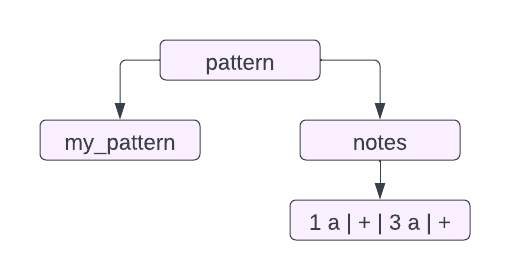
\includegraphics[scale=0.8]{Copy of Blank diagram-2.png}


	AST for example 2:
    
    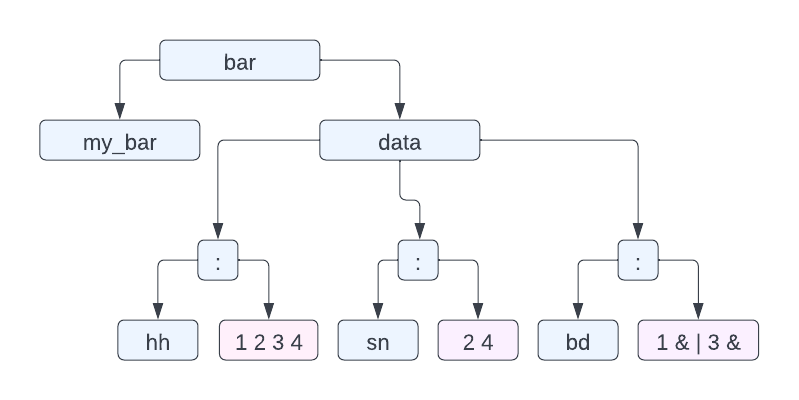
\includegraphics[scale=0.8]{Copy of Copy of Blank diagram.png}

	AST for example 3: (note that I've omitted the implementation of "my bar" as it is similar to example 2)
    
    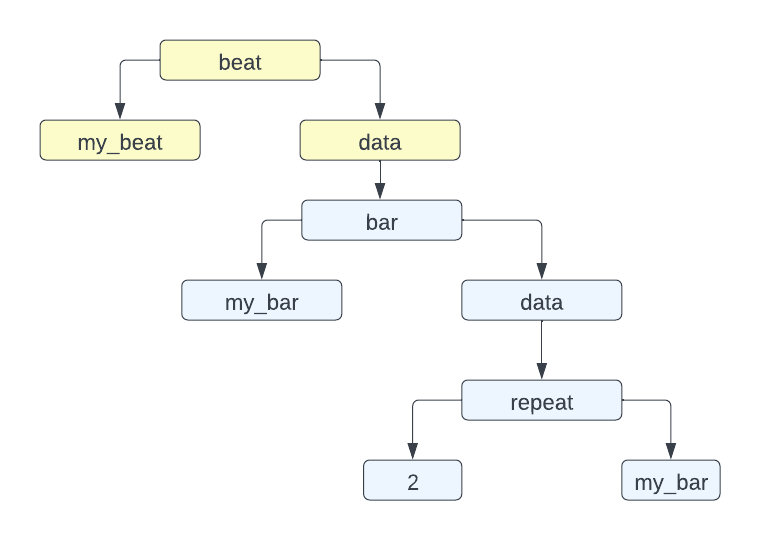
\includegraphics[scale=0.8]{Copy of Blank diagram.png}


    \item 
        \begin{enumerate}[A.]
        \item The programs do not read input.
        \item The output is a pdf file. 
        \item Evalution of the program illustrated by example 2. First we evaluate the left branch, which is name
		of the bar. The we evaluate the right branch which contains actions as children. Each action has a drum name 
		as the left node and a pattern as the right node. We first evaluate the drum, and then the pattern and assign
		the pattern to the drum. We continue doing so until we evaluate every action. 

		
		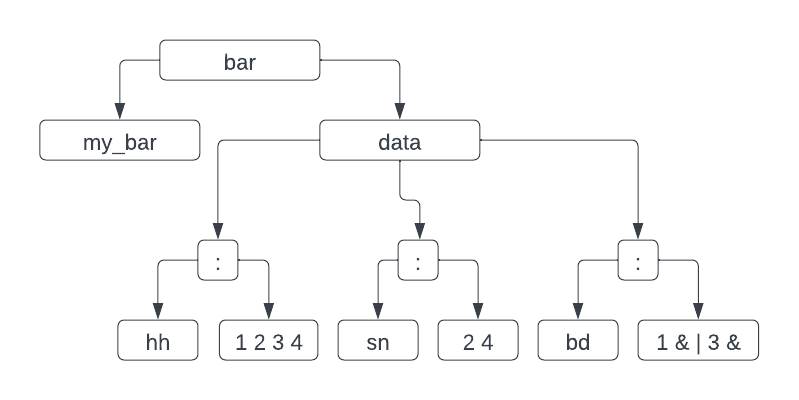
\includegraphics[scale=0.6]{Copy of Copy of Blank diagram-9.png}
		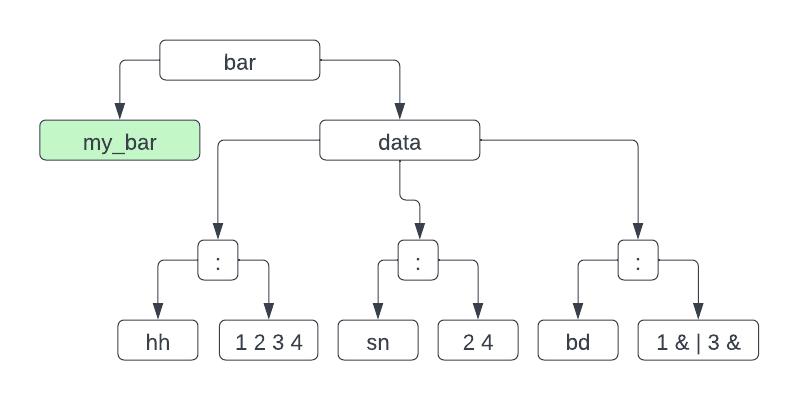
\includegraphics[scale=0.6]{Copy of Copy of Blank diagram-10.png}
		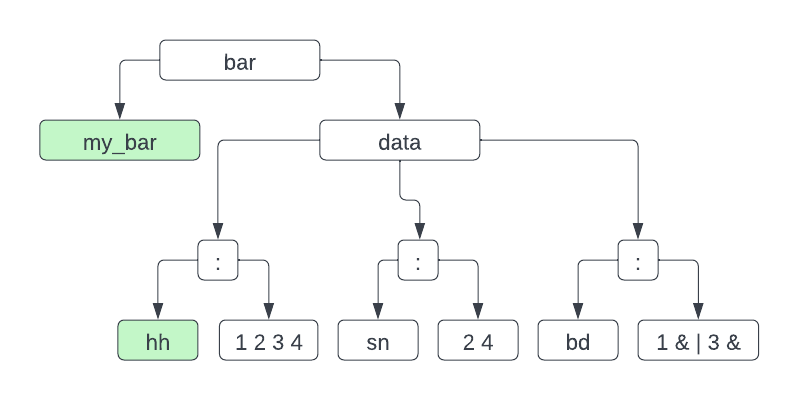
\includegraphics[scale=0.6]{Copy of Copy of Blank diagram-11.png}
		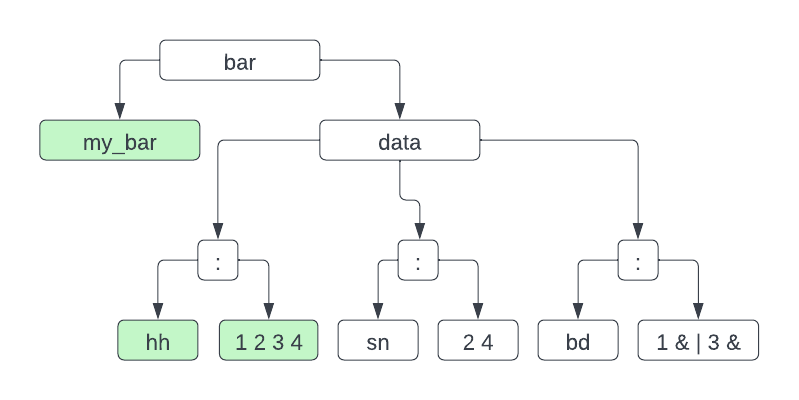
\includegraphics[scale=0.6]{Copy of Copy of Blank diagram-12.png}
		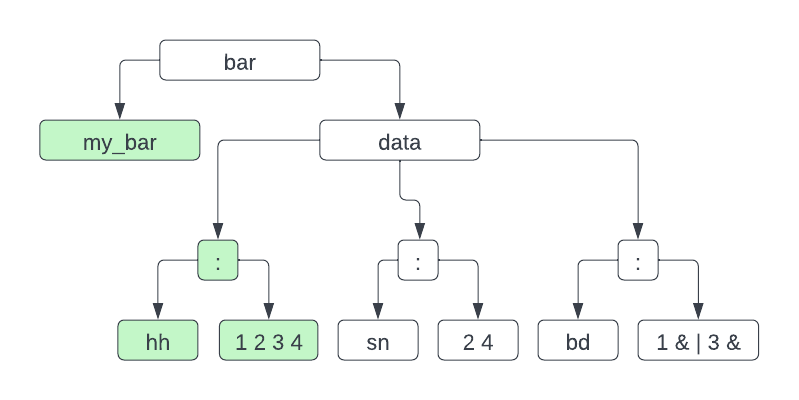
\includegraphics[scale=0.6]{Copy of Copy of Blank diagram-13.png}
		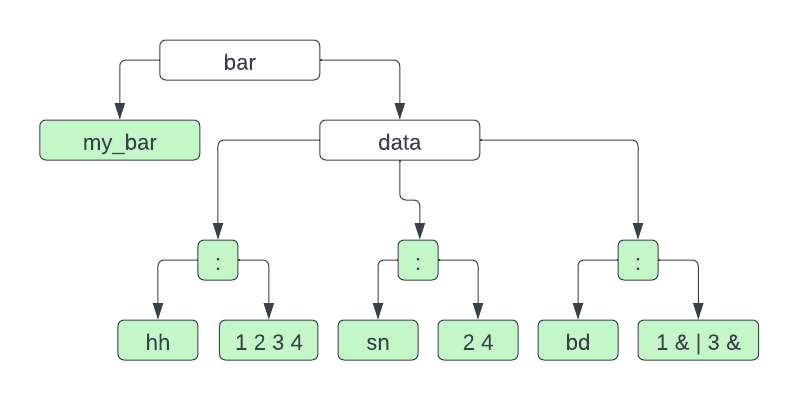
\includegraphics[scale=0.6]{Copy of Copy of Blank diagram-14.png}
		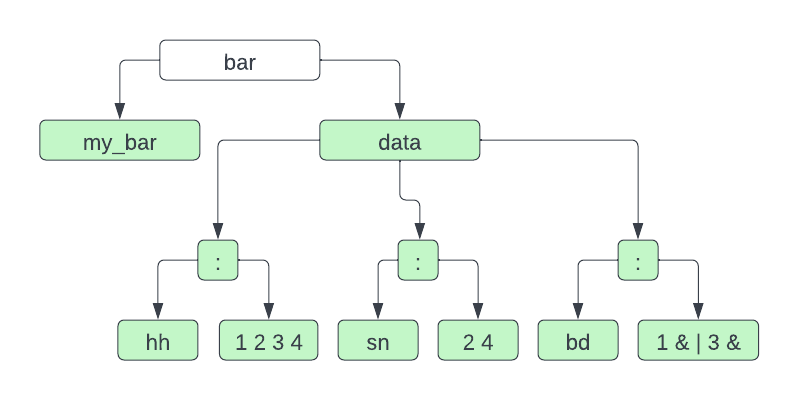
\includegraphics[scale=0.6]{Copy of Copy of Blank diagram-15.png}
		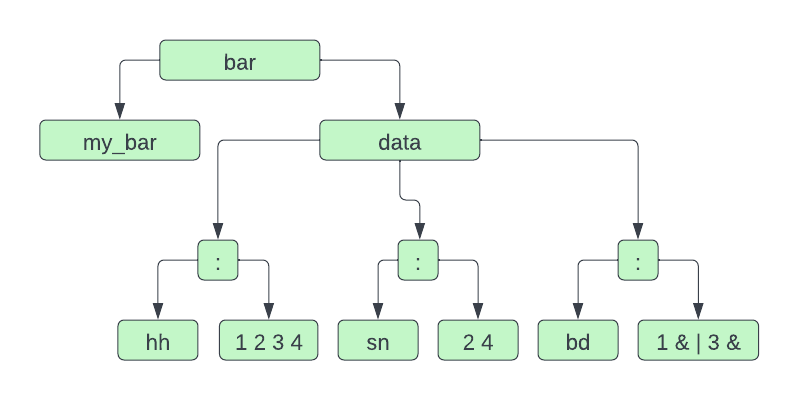
\includegraphics[scale=0.6]{Copy of Copy of Blank diagram-16.png}


        \end{enumerate}
    
\end{enumerate}

% DO NOT DELETE ANYTHING BELOW THIS LINE
\end{document}